\documentclass[a4paper,12pt]{article}
\usepackage[utf8]{inputenc}
\usepackage[spanish]{babel}
\usepackage{color}
\usepackage{parskip}
\usepackage{graphicx}
\usepackage{multirow}
\usepackage{listings}
\definecolor{mygreen}{rgb}{0,0.6,0}
\definecolor{lbcolor}{rgb}{0.9,0.9,0.9}

\lstset{
backgroundcolor=\color{lbcolor},
    tabsize=4,    
%   rulecolor=,
    language=[GNU]C++,
        basicstyle=\tiny,
        aboveskip={1.5\baselineskip},
        columns=fixed,
        showstringspaces=false,
        extendedchars=false,
        breaklines=true,
        prebreak = \raisebox{0ex}[0ex][0ex]{\ensuremath{\hookleftarrow}},
        frame=single,
        showtabs=false,
        showspaces=false,
        showstringspaces=false,
        identifierstyle=\ttfamily,
        keywordstyle=\color[rgb]{0,0,1},
        commentstyle=\color[rgb]{0.026,0.112,0.095},
        stringstyle=\color{red},
        numberstyle=\color[rgb]{0.205, 0.142, 0.73},
%        \lstdefinestyle{C++}{language=C++,style=numbers}’.
}

\begin{document}

\twocolumn[

\begin{@twocolumnfalse}
\section{Problema}

En un archivo de texto plano se tine una cola de trabajos esperando su impresión.
El planificador del servicio de impresión decide atender segun la cantidad de hojas
Su política es de imprimir los trabajos que tienen menos hojas. Realice un programa que ayude al
servicio de impresión a establecer la orden de impresión utilizando la estructura de datos Montículo.\\ \\

\end{@twocolumnfalse}
]
\section{Código}

\subsection{Monticulo.h}

\begin{lstlisting}

#ifndef MONTICULO_H
#define MONTICULO_H
#include <vector>
#include <iostream>
using namespace std;

class Monticulo
{
    public:
        Monticulo();
        virtual ~Monticulo();
        void ingresar(int);
        void print();
        int size();
        int del();
    protected:
    private:
        vector<int> monti;
};

Monticulo::Monticulo(){}
Monticulo::~Monticulo(){}

int Monticulo::size(){
    return monti.size();
}

int Monticulo::del(){
    int resultado = monti.front();
    if(monti.size() == 0)return resultado;
    monti[0] = monti[monti.size() - 1];
    monti.pop_back();
    int pos = 0;
    while(pos <= monti.size() - 1){
        if(2 * pos + 1 > monti.size() - 1)return resultado;
        if(2 * pos + 2 > monti.size() - 1){
            if(monti[pos] > monti[2 * pos + 2]){
                auto temp = monti[pos];
                monti[pos] = monti[2 * pos + 2];
                monti[2 * pos + 2] = temp;
                return resultado;
            }
        }
        if(monti[pos] > monti[2 * pos + 1] or monti[pos] > monti[2 * pos + 2]){
            if(monti[2 * pos + 1] < monti[2 * pos + 2]){
                auto temp = monti[pos];
                monti[pos] = monti[2 * pos + 1];
                monti[2 * pos + 1] = temp;
                pos = 2 * pos + 1;
            }
            else{
                auto temp = monti[pos];
                monti[pos] = monti[2 * pos + 2];
                monti[2 * pos + 2] = temp;
                pos = 2 * pos + 2;
            }
        }
        else{
            break;
        }
    }
    return resultado;
}

void Monticulo::print(){
    for(int i = 0; i < monti.size(); i++){
        cout<<monti[i]<<endl;
    }
}

void Monticulo::ingresar(int valor){
    monti.push_back(valor);
    int pos = monti.size() - 1;
    while(pos > 0){
        if(monti[pos] < monti[(pos - 1) / 2]){
            auto temp = monti[pos\onecolumn];
            monti[pos] = monti[(pos - 1) / 2];
            monti[(pos - 1) / 2] = temp;
        }
        pos = (pos - 1) / 2;
    }
}

#endif // MONTICULO_H

\end{lstlisting}
\newpage

\subsection{Main.cpp}

\begin{lstlisting}
#include <iostream>
#include "Monticulo.h"
#include <fstream>
#include "math.h"
using namespace std;

float convertirNumero(string numero){
    double resultado = 0;
    auto iter = numero.end();
    iter--;
    double contador = 0;
    for(iter; iter!= numero.begin(); iter--){
        if((*iter) == '.'){
            resultado /= pow(10,contador);
            contador = -1;
        }
        else{
            resultado += pow(10,contador) * ((*iter) - 48);
        }
        contador++;
    }
    resultado += pow(10,contador) * ((*iter) - 48);
    return resultado;
}

bool esNumero(string::iterator &letra){
    if(*letra >= 48 and *letra <= 57)return true;
    return false;
}

float verificarLinea(string linea){
    int estado = 0;
    string resultado;
    for(auto iter = linea.begin(); iter != linea.end(); ++iter){
        if(estado == 5)break;
        switch(estado){
            case 0:
                if(*iter == 116)estado = 1;
                else return -1;
                break;
            case 1:
                if(esNumero(iter))estado = 2;
                else return -1;
                break;
            case 2:
                if(esNumero(iter))estado = 2;
                else if(*iter == 32)estado = 3;
                else return -1;
                break;
            case 3:
                if(esNumero(iter)){
                    estado = 4;
                    resultado.insert(resultado.end(),*iter);
                }
                else return -1;
                break;
            case 4:
                if(esNumero(iter)){
                    estado = 4;
                    resultado.insert(resultado.end(),*iter);
                }
                else if(*iter == 32) estado = 5;
                else return -1;
                break;
            default:
                return -1;
        }
    }
    return convertirNumero(resultado);
}

int main()
{
    Monticulo impresion;
    ifstream archivo("hojas.txt");
    if(archivo.fail()){
        cout<<"No se pudo abrir el archivo"<<endl;
        return 0;
    }t1 7 hojas
t2 15 hojas
t3 4 hojas
t4 20 hojas
    char linea[128];
    int numberLine = 0;
    while(archivo.getline(linea,128)){
        numberLine++;
        string tempLinea(linea);
        auto number = verificarLinea(tempLinea);
        if(number == -1){
            cout<<"Error en la linea "<<numberLine<<endl;
        }
        else{
            impresion.ingresar(number);
        }
    }
    archivo.close();
    auto tam = impresion.size();
    for(int i = 0; i < tam; i++){
        cout<<"Impresion numero "<<i+1<<" :"<<impresion.del()<<" hojas"<<endl;
    }
}

\end{lstlisting}



\onecolumn

\section{Ejemplos}

Para probar el programa, se utilizó un archivo de texto plano llamado ``hojas.txt'' con el siguiente contenido:



\begin{itemize}
 \item t1 7 hojas
\item t2 15 hojas
\item t3 4 hojas
\item t4 20 hojas
\end{itemize}

\begin{figure}[h]
 \centering
 \includegraphics[scale=0.5]{imagenes/1.eps}
 \caption{Ejemplo}
\end{figure}
\end{document}